\documentclass[a4paper,12pt]{book}
\usepackage{amsmath, amsthm}
\usepackage{datetime}
\usepackage{framed}
\usepackage{enumitem}
\usepackage{fancyref}
\usepackage{wrapfig}
\usepackage{pifont}
\usepackage{appendix}
\usepackage{caption}
\usepackage{xcolor}
\usepackage[stable]{footmisc}
\usepackage{multicol}
\usepackage{csquotes}
\usepackage{pdfpages}

\usepackage{amsthm}

\usepackage{amssymb}
\usepackage{amsfonts}
\usepackage{mathtools}

\usepackage{eso-pic}

\usepackage{tikz}
\usepackage{pgf}
\usepgflibrary{fpu}
\usepackage{qtree}
\usetikzlibrary{angles,fit,arrows,calc,math,intersections,through,backgrounds,cd}
\usepackage{pgfplots}
\usepackage{tkz-euclide}

\usepackage{listings}
\usepackage{graphicx}
\usepackage{wasysym}
\usepackage{hyperref}
\lstset{
    basicstyle=\itshape,
    xleftmargin=3em,
    literate={->}{$\rightarrow$}{2}
{α}{$\alpha$}{1}
{δ}{$\delta$}{1}
}


\usepackage{csquotes}
\renewcommand{\mkbegdispquote}[2]{\itshape}

\newdateformat{nianyueri}{修订于 \THEYEAR 年 \THEMONTH 月 \THEDAY 日 }


\usepackage{quiver}
\usepackage{circledsteps}
\usepackage[top=1in,bottom=1in,left=1in,right=1in]{geometry} % 用于设置页面布局
\usepackage{xeCJK} % 用于使用本地字体
\usepackage[super, square, sort&compress]{natbib} % 处理参考文献
\usepackage{titlesec, titletoc} % 设置章节标题及页眉页脚
\usepackage{amssymb}
\usepackage{amsmath} % 在公式中用\text{文本}输入中文
\usepackage{diagbox}
\usepackage{multirow} % 表格中使用多行
\usepackage{booktabs} % 表格中使用\toprule等命令
\usepackage{rotating} % 使用sidewaystable环境旋转表格
\usepackage{tabularx}
\usepackage{graphicx} % 处理图片
\usepackage{footnote} % 增强的脚注功能,可添加表格脚注
\usepackage{threeparttable} % 添加真正的表格脚注,示例见README
\usepackage{hyperref} % 添加pdf书签

\usepackage{tikz}
\usetikzlibrary{shapes,arrows,shadows}


% 字体设置
\setmainfont{Times New Roman}
\setsansfont[Scale=MatchLowercase,Mapping=tex-text]{PT Sans}
\setmonofont[Scale=MatchLowercase]{PT Mono}
\setCJKmainfont[ItalicFont={FZKai-Z03}, BoldFont={FZHei-B01}]{FZShuSong-Z01}
\setCJKsansfont{FZHei-B01}
\setCJKmonofont{FZShuSong-Z01}

\newcommand{\song}{\CJKfamily{song}} % 宋体
\newcommand{\fs}{\CJKfamily{fs}} % 仿宋体
\newcommand{\kai}{\CJKfamily{kai}} % 楷体
\newcommand{\hei}{\CJKfamily{hei}} % 黑体
\newcommand{\li}{\CJKfamily{li}} % 隶书
\newcommand{\you}{\CJKfamily{you}} % 幼圆
\def\songti{\song}
\def\fangsong{\fs}
\def\kaishu{\kai}
\def\heiti{\hei}
\def\lishu{\li}
\def\youyuan{\you}

%%设置常用中文字号,方便调用
\newcommand{\chuhao}{\fontsize{42pt}{\baselineskip}\selectfont}
\newcommand{\xiaochu}{\fontsize{36pt}{\baselineskip}\selectfont}
\newcommand{\yihao}{\fontsize{26pt}{\baselineskip}\selectfont}
\newcommand{\xiaoyi}{\fontsize{24pt}{\baselineskip}\selectfont}
\newcommand{\erhao}{\fontsize{22pt}{\baselineskip}\selectfont}
\newcommand{\xiaoer}{\fontsize{18pt}{\baselineskip}\selectfont}
\newcommand{\sanhao}{\fontsize{16pt}{\baselineskip}\selectfont}
\newcommand{\xiaosan}{\fontsize{15pt}{\baselineskip}\selectfont}
\newcommand{\sihao}{\fontsize{14pt}{\baselineskip}\selectfont}
\newcommand{\xiaosi}{\fontsize{12pt}{\baselineskip}\selectfont}
\newcommand{\wuhao}{\fontsize{10.5pt}{\baselineskip}\selectfont}
\newcommand{\xiaowu}{\fontsize{9pt}{\baselineskip}\selectfont}
\newcommand{\liuhao}{\fontsize{7.5pt}{\baselineskip}\selectfont}
\newcommand{\xiaoliu}{\fontsize{6.5pt}{\baselineskip}\selectfont}
\newcommand{\qihao}{\fontsize{5.5pt}{\baselineskip}\selectfont}
\newcommand{\bahao}{\fontsize{5pt}{\baselineskip}\selectfont}

% 章节标题显示方式及页眉页脚设置
% \item xCJKnumb是自己额外安装的包
% \item titleformat命令定义标题的形式
% \item titlespacing定义标题距左、上、下的距离
\titleformat{\section}{\raggedright\large\bfseries}{\thesection}{1em}{}
\titleformat{\subsection}{\raggedright\normalsize\bfseries}{\thesubsection}{1em}{}
\titlespacing{\section}{0pt}{*2}{*0}
\titlespacing{\subsection}{0pt}{*1}{*0}

% 由于默认的2em缩进不够,所以我手动调整了,但是在windows下似乎2.2就差不多了,或者是article中没有这个问题
\setlength{\parindent}{0em}
\setlength{\parskip}{0.25em}

% 设置表格标题前后间距
\setlength{\abovecaptionskip}{0pt}
\setlength{\belowcaptionskip}{0pt}

% 设置列表项目前后间距
\setlength\itemsep{0em}

\renewcommand{\refname}{\bfseries{参~考~文~献}} %将Reference改为参考文献(用于 article)
% \renewcommand{\bibname}{参~考~文~献} %将bibiography改为参考文献(用于 book)

\renewcommand{\baselinestretch}{1.4} %设置行间距
\renewcommand{\figurename}{\small\ttfamily 图}
\renewcommand{\tablename}{\small\ttfamily 表}


\usepackage{stmaryrd}
\usepackage{mathtools}
\usepackage{wasysym}
\usepackage{textcomp}
\usepackage{blindtext}
\usepackage{subfiles}

\newtheorem{problem}{问题}
\numberwithin{problem}{section}
\newtheorem{definition}{定义}
\numberwithin{definition}{section}
\newtheorem{lemma}{引理}
\numberwithin{lemma}{section}
\newtheorem{proposition}{命题}
\numberwithin{proposition}{section}
\newtheorem{theorem}{定理}
\numberwithin{theorem}{section}
\newtheorem{grammar}{文法}
\numberwithin{grammar}{section}
\newtheorem{program}{程序}
\numberwithin{program}{section}
\newtheorem{convention}{约定}
\numberwithin{convention}{section}
\newtheorem{corollary}{推论}
\numberwithin{corollary}{section}
\renewcommand*{\proofname}{证明}

\xeCJKsetwidth{‘’“”}{1em}

\newcommand{\specialcell}[2][c]{%
\begin{tabular}[#1]{@{}c@{}}#2\end{tabular}}

\titleformat{\chapter}[display]
{\bfseries \sanhao}
{第 \thechapter 章}
{1ex}
{\titlerule\vspace{1ex}\filleft}
[\vspace{1ex}\titlerule]

\titlespacing{\chapter}{0pt}{*1}{*1.5}

\title{算术表达式的几何}
\date{\nianyueri\today}
\author{苑明理}

\begin{document}

\begin{titlepage}
\centering{\AddToShipoutPictureBG*{\AtPageLowerLeft{\includegraphics[width=\paperwidth,height=\paperheight]{../images/seaside-footprint.png}}}}
\centering{\erhao 算术表达式的几何}\\
\vspace{10mm}
\vspace{\fill}
\centering{\sihao 苑明理 \\ \wuhao 修订于 2024 年 8 月 19 日}

\end{titlepage}

\newpage
\thispagestyle{empty}

\frontmatter
\thispagestyle{empty}

\newpage
\thispagestyle{empty}
\vspace*{2cm}
\begin{center}
\parbox{10cm}{\wuhao \em 我们在未知的海岸边发现了一串奇怪的脚印......\flushright— 亚瑟·爱丁顿}
\end{center}

\newpage
\thispagestyle{empty}

\centerline{\rule{13cm}{0.4pt}}
\renewcommand{\contentsname}{\hfill\bfseries 目录\hfill}
\setcounter{tocdepth}{2}
\tableofcontents
\centerline{\rule{13cm}{0.4pt}}

\mainmatter

\setlength{\parindent}{0em}
\setlength{\parskip}{1.2em}
\setcounter{page}{1}

\chapter{研究的开端}

我深知自己智力的有限,然而,当那些迷人的问题逐一浮现,更多的可能性渐渐清晰,我站在了一个分岔口:是否应该扬帆驶向那片未知的海域?
在 2022 年初春,我做出了选择—启航。虽说这份文档的每一章节都还有未解开的谜题,在两年的梳理与探求后,我已能够用更加严密的语言去阐述这些问题了。
因此,我诚挚邀请诸位同行去共同探寻那神秘的海域。

\section{词向量的正则性}

我们的探索可以从 2013 年讲起,当时自然语言处理领域逐步发展出了词嵌入技术,引发大量关注与研究。词嵌入最吸引人的地方在于,词向量可以捕捉到词语之间的语义关系,
使得一种之前没见过的“正则性”(regularity)成立。这种正则性指出,两对词语在语义上的相似性,对应到几何上有词向量之间的平行性。
所以,它把词语的同义关系给以几何化表达,赋予了空间维度以语义。

\begin{figure}
\centering
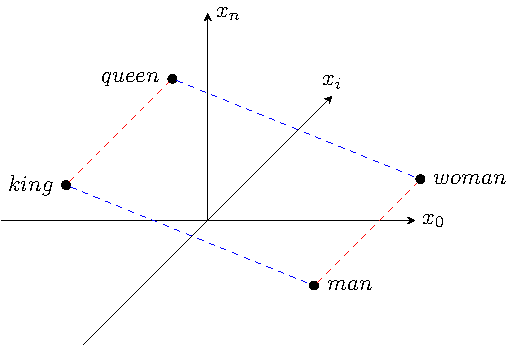
\includegraphics{../images/wordembedding}
\caption{词向量的正则性}
\end{figure}

最为著名的例子是“男人”、“女人”、“国王”和“王后”之间的关系,让我们对它稍作解析。

从上图我们可以看到四个嵌入的点和两组平行关系:

\colorbox{red!10}{
性别维度:男人 $-$ 女人 ≈ 国王  $-$ 女王
}
\\
\colorbox{blue!10}{
王权维度:国王 $-$ 男人 ≈ 女王  $-$ 女人
}

两组平行关系形成一个平行四边形。我们改写一下,得到端点和关系的运算:

\colorbox{yellow!10}{男人 + 性别维度移动 + 王权维度移动 = 女王}
\\
\colorbox{yellow!10}{男人 + 王权维度移动 + 性别维度移动 = 女王}

或者说,这反映了关系运算满足交换律:

\colorbox{yellow!10}{性别维度移动 + 王权维度移动 = 王权维度移动 + 性别维度移动}

在下一节里,我们能看到,这里对关系的正则性形式进行的改写,会帮助我们从新的角度理解问题。

然而,在 2013 年和随后几年,技术发展没有沿着正则性的角度继续前进,而是转向了更加复杂的各种自然语言任务和语言模型。
尽管如此,我思考的起点却是从这里延伸出来——如果我们把这种关系正则性强制要求下来,会发生什么呢?

\section{数字的双曲表示}

2015 年的秋天,我拿数字和数字的运算关系做了一些实验,尝试把正则性强制要求下来,但很快就发现这里面存在一些困难。
让我们举例子来说明一下,我们考察简单的“$+1$”和“$\times 2$”的关系。

此时,所有的数字都映射为空间的点,而“$+1$”和“$\times 2$”运算关系映射为空间中的向量。假设从一个点 $\alpha$ 出发,我们可以进行一系列的运算关系组合,比如:
\begin{itemize}
\item 先“$+1$”再“$\times 2$”操作:$(\alpha +1) \times 2 = 2 \alpha + 2$
\item 先“$\times 2$”再“$+1$”操作:$\alpha \times 2 + 1 = 2 \alpha + 1$
\end{itemize}

于是,不论我们从哪个点出发,这两个运算关系都不具备交换性,所以它们无法形成平行四边形。

平行四边形可以在两次关系运算的组合中约化掉其中一个,从而可以避免运算关系组合的指数爆炸。
而平行四边形无法形成,这意味着运算关系组合的指数爆炸无法避免。

\begin{figure}
\centering
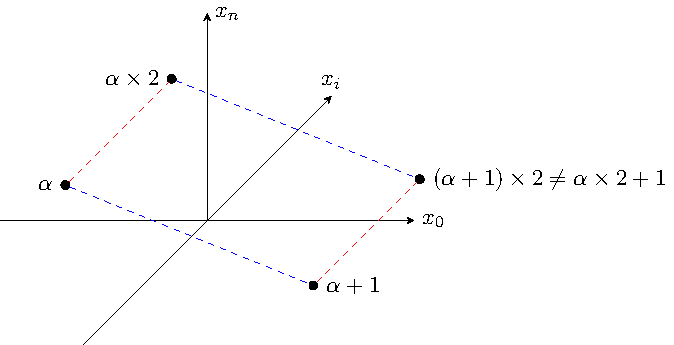
\includegraphics{../images/numberembedding}
\caption{数字嵌入遇到的矛盾}
\end{figure}

如果每个特征在表征空间里都占据有限大的体积,且这个有限大的体积存在一个最小的分辨限制,那么组合爆炸就意味着我们需指数增长的体积来容纳这些运算关系的组合。
在欧式空间里,球体的体积随着半径增长是多项式级别增长的,所以随着表达式数量的增加,表征空间会很快不足够使用。

幸运的是,几何学里有一种空间,它的容量是指数增长的,同时它里面也不存在平行四边形构造,这就是双曲空间。我决定拿双曲空间来尝试解决这个问题。
\footnote{所有关系运算的可能组合的数量是一种复杂性度量,于是整个讨论隐含了体积或者面积正比于这个度量。这个观点在后面计算\ref{chap:computation}的时空复杂性里还会有所阐发。}

\begin{figure}[ht]\centering
\resizebox{0.5\textwidth}{!}{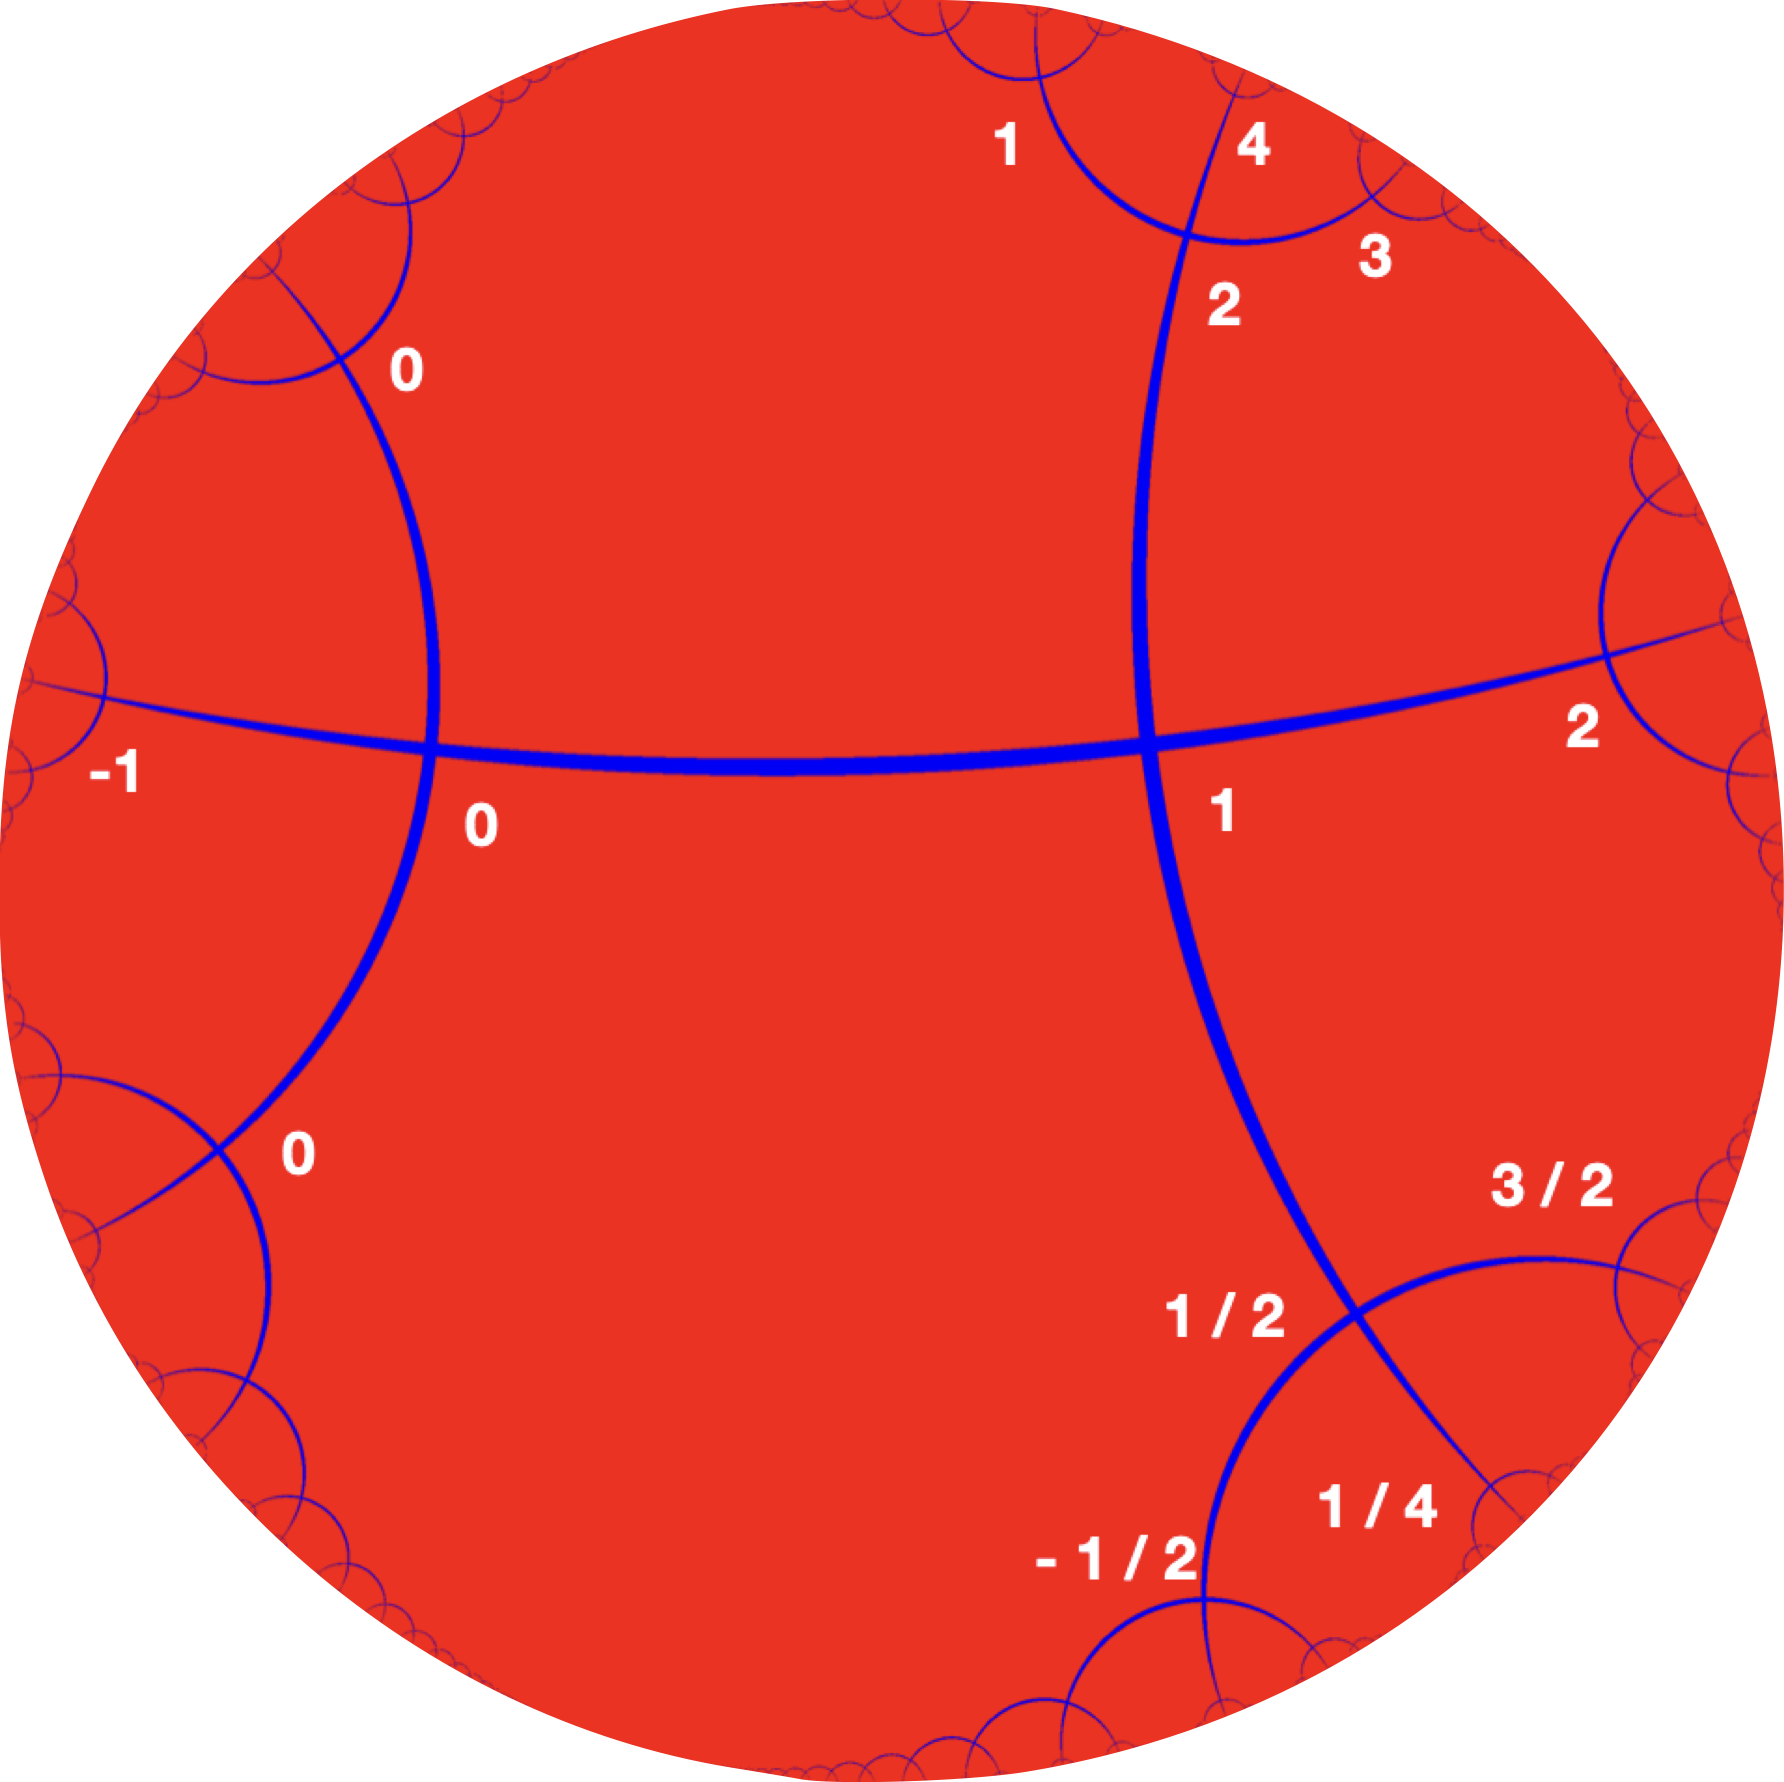
\includegraphics{../images/assignment2}}
\caption{庞加莱圆盘上的加乘与数字安排}\label{fig:assignment2}
\end{figure}

经过一些尝试,我很快就发现,一种称之为四阶无限边形铺嵌的结构可以用来编码一些数字的加法和乘法。如图 \ref{fig:assignment2},横着的最主要的那根轴是加法轴,
数字按照加法的规律从左到右不断加一排布;与之垂直的轴是乘法轴,数据按照乘法的规律逐步乘二排布。与乘法轴垂直的都是加法轴,而与加法轴垂直的都是乘法轴。
通过这种加乘交错的构造我们可以编码数字的加法和乘法运算。

当这个数字的四阶无限边形排布做出来以后,望着这些高度对称分布的点值,我产生了非常自然的一个疑问\footnote{最初的这个问题,至今还没有完全解决。},这些离散点值能否连续扩展到整个庞加莱圆盘?
如果这些点值能连续的分布在整个庞加莱圆盘上,那么我们就可以用它来编码所有实数值的算术运算了。

\section{流方程的引入}

时间飞逝到了 2019 年,我在出差的飞机上,突然想到既然我希望这些点值能够连续的分布在整个庞加莱圆盘上,那么为什么我不试一下无穷小的生成过程呢?
我在飞机上快速做了一些推导,结果是正面的。旅途结束后的几天,我就得到了一个微分方程,它描述了一个加法生成元$\mu$和乘法生成元$e^\lambda$的双生成元无穷小生成过程。

假设我们有一个基点 $a_0$,然后我们从 $a_0$ 走一小段距离。$\epsilon$ 是一个小的距离量,$\delta$ 是一个小的时间量。
移动同加法的坐标轴的夹角是 $\theta$,于是$\mu \epsilon \cos \theta$是加法生成元的贡献,$e^{\lambda \epsilon \sin \theta}$是乘法生成元的贡献。

对于优先加法的情形,我们有

\[
a_{\delta} = (a_0 + \mu \epsilon \cos \theta)e^{\lambda \epsilon \sin \theta}
\]

对于优先乘法的情形,我们有

\[
a_{\delta} = a_0 e^{\lambda \epsilon \sin \theta} + \mu \epsilon \cos \theta
\]

略去高阶小项,两种情形都可以简化为同一个结果:

\[
a_{\delta} = a_0 + \epsilon (a_0 \lambda \sin \theta + \mu \cos \theta)
\]

所以我们有如下的方程

\[
\frac{1}{\delta} (a_{\delta} - a_0) = \frac{\epsilon}{\delta} (\mu \cos \theta + a_0 \lambda \sin \theta)
\]

当 $\delta$ 和 $\epsilon$ 同时趋近于零,我们得到 $da / dt$,于是有

\[
\frac{da}{dt} = u (\mu \cos \theta + a \lambda \sin \theta)
\]

此处,$u$ 是 $\epsilon / \delta$ 的极限值。 或者,我们把$u$移动到左边的分母上,取 $ds = u dt$ ,改写成如下的形式

\begin{equation}
\frac{da}{ds} = \mu \cos \theta + a \lambda \sin \theta\label{eq:flow}
\end{equation}

整个推导非常初等,只涉及极限过程和微元的基本运算。因为这个方程刻画了一个计算的流动过程,所以我称之为“流方程”。
流方程是可解的,解刻画了一个连续生成过程,再稍微分析一下就可以发现这个连续生成过程里容纳一个离散生成过程。
它反映了连续和离散两种生成过程的融洽性,这一点我们会在后面的章节里详细讨论。

\section{第一个解析解}

\begin{figure}[ht]\centering
\resizebox{0.8\textwidth}{!}{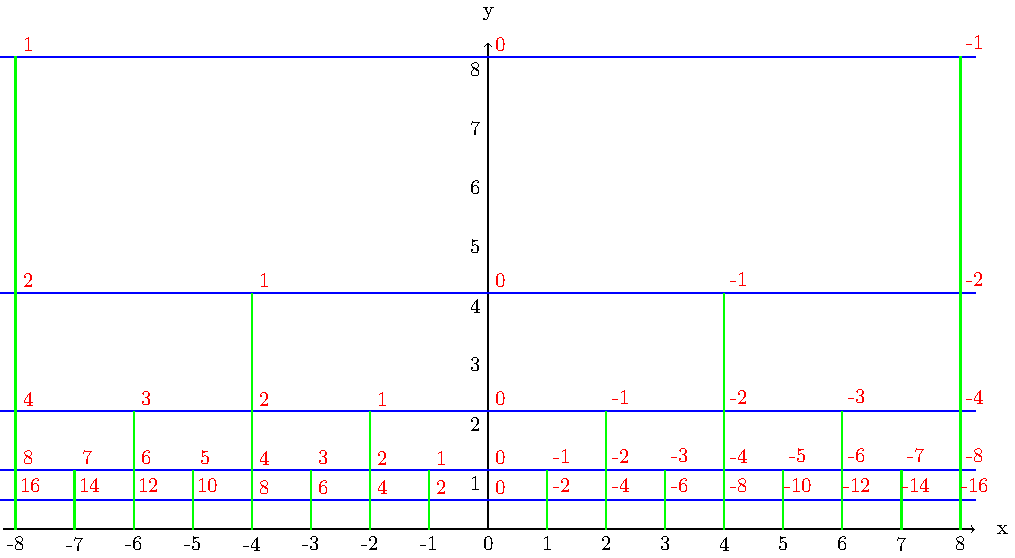
\includegraphics{../images/01-grid-example-1}}
\caption{上半平面模型里的加乘与数字安排}\label{fig:assignment1}
\end{figure}

2021 年春天,我得到公司(彩云科技)的支持,和两个实习生一起工作了三个月,做了一些更加严谨的研究。来自山东大学的张乐同学利用分离变量法很快推导出了两个流方程的解析解。
我们经过研究,发现两个解析解本质上是同一个。在上半平面模型里,只要能分离变量,
不论加法生成元 $\mu$ 还是乘法生成元 $e^\lambda$ 的取值怎么变化,我们只需要变化空间的度规,
赋值场 $a$ 始终是同一个解析解$a = - \frac{x}{y}$。

在这个解析解之前,我们仅有一些猜测,比如庞加莱圆盘里的四阶无限边形结构,它只是知道离散结构,但不知道连续结构。
而张乐给出的解析解,让我们第一次有了一个可以仔细研究的严格数学对象。我经过一些尝试,画出了这个解析解的图像代表它的离散生成关系,
它是一种称为 Baumslag–Solitar 群的特例。

在上图中,我们首先可以看到一些红色的离散点值$a$,它们符合解析式 $a = -\frac{x}{y}$。
蓝横线是伪圆,它们从右向左按照加一的规律不断增长,代表了一条条的加法轴。绿竖线是测地线,它们从上向下按照乘二的规律不断增长,代表了一条条的乘法轴。
蓝横线和绿竖线交错排布,彼此垂直。

\begin{figure}[ht]\centering
\resizebox{0.8\textwidth}{!}{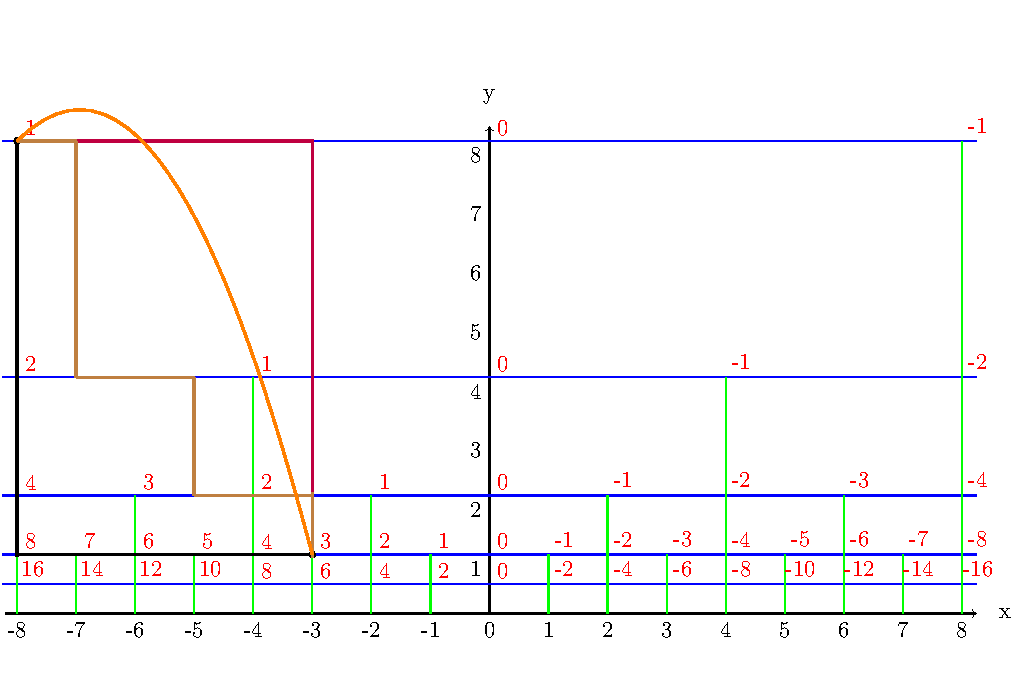
\includegraphics{../images/encoding}}
\caption{路径编码算术表达式}\label{fig:encoding}
\end{figure}

因为蓝横线和绿竖线交错的网格的存在,我们可以利用它来编码一些数值的算术运算。比如 $1 \times 8 - 5 = 3$,我们可以在网格上画出这个算术运算的路径。
从任何一个 $a$ 值为 $1$ 的点出发,向下走三步,完成三次乘二操作,然后向右走五步,完成减五的操作,就会到达一个 $a$ 值为 $3$ 的点,也就是上图中黑色的线。

完全类似的,上图中紫红色的线编码了 $(1 - \frac{5}{8}) \times 8 = 3$ 的算术运算;
褐色的线编码了 $(((1 - \frac{1}{8}) \times 2 - \frac{2}{4}) \times 2 - 1) \times 2 = 3$ 的算术运算。

上面的例子都是折线,那么有趣的问题是橙色的曲线编码了什么?仔细考虑一下,就会意识到它编码了一种特别的、不同于传统的黎曼积分的积分过程。黎曼积分只是累加小量;
而这个曲线代表的积分过程会同时累加小量和累乘小量,加法的小量是指趋近于零的量,而乘法的小量是指趋近于一的量。

\newpage

\chapter{基本概念}

本节我们作更加严格的论述,引入一些基本概念,为后继的讨论进行铺垫。在此,我们需要指出,算术表达式的几何有两种不同的研究途径,有不同的趣旨和目标。
一种是构造性的途径,它试图通过特定的定义和构造方式,一步步的从离散的有理数域的表达式,构造出实数域的表达式,并形成一个几何空间。
另一种是解释性的途径,它试图通过微积分的工具,直接在几何空间上讨论一个标量场$a$,称为赋值场,这个场满足流方程,可以把一些折线路径解释为离散的算术表达式,
甚至扩展至一种特殊的加乘积分构造。这两种不同的途径都是我们研究的方法。

\section{算术表达式}\label{sec:arithmetic-expression}

从计算机科学的角度来看,算术表达式是一种抽象的递归数据类型,它可以被解析成为一棵树。这棵树的叶子节点是操作数,内部节点是操作符。
所以也可以说,算术表达式有字串表示和树表示两种形式,常见的形式是字串表示,基于中缀表示法和括号的优先级规则。

比如,对于表达式

\begin{equation}
(((((1 \times 2) \times 2) - 1) \times (2 + 1)) - 6)
\end{equation}

我们有如下的解析树

\begin{figure}[ht]
\centering
\resizebox{0.3\textwidth}{!}{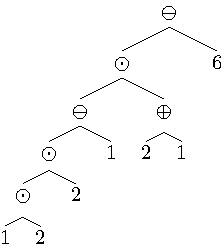
\includegraphics{../images/02-example-expression-syntax-tree.pdf}}
\caption{表达式的解析树}\label{fig:syntaxtree}
\end{figure}

我们尝试在有理数域 $Q$ 上给出算术表达式的定义。这是一种生成式的递归定义方式,它说明:有理数本身可以构成算术表达式;算术表达式的加、减、乘、除组合仍然构成算术表达式。

\begin{definition}\label{def:arithmetic-expression}
数域 $\mathbb{Q}$ 上的算术表达式 $a$ 是被如下生成式定义的结构
\begin{equation}\label{eq:productionrule}
\begin{aligned}
a &\longleftarrow x\\
a &\longleftarrow ( a + a )\\
a &\longleftarrow ( a - a )\\
a &\longleftarrow ( a \times a )\\
a &\longleftarrow ( a \div a )
\end{aligned}
\end{equation}
其中 $x \in \mathbb{Q}$,我们把所有算术表达式写成$\mathbb{E} \left [\mathbb{Q} \right ]$,且有 $a \in \mathbb{E} \left [\mathbb{Q} \right ]$.
\end{definition}

纯数学专业的读者可能会不熟悉这种定义方式,可以参考形式语言里的生成式定义,我们这里终止符号是有理数、括号和四则运算符号,非终止符号是表达式。

在这个递归生成结构上也可以递归定义一个求值的过程 $\nu(a)$,可以理解成表达式树表示上的一种遍历过程。

\begin{itemize}
\item 常数叶节点: 对 $x \in \mathbb{Q}$, 有 $\nu(x) = x$.
\item 加法节点 $+$: 对 $(a + b)$, 有 $\nu((a + b)) = \nu(a) + \nu(b)$.
\item 减法节点 $-$: 对 $(a - b)$, 有 $\nu((a - b)) = \nu(a) - \nu(b)$.
\item 乘法节点 $\times$: 对 $(a \times b)$, 有 $\nu((a \times b)) = \nu(a) \nu(b)$.
\item 除法节点 $\div$: 对 $(a \div b)$,若 $\nu(b) \neq 0$, 有 $\nu((a \div b)) = \nu(a) / \nu(b)$.
\end{itemize}

细心的读者可能已经注意到,我们的算术表达式时是定义在有理数域上的,为什么不能直接定义在实数域呢。原因是我们在定义表达式的除法时,必须要求除数不为零。
而在有理数域上,一个子表达式是否为零是可以判定的。在实数域上,表达式是否为零不可判定的。\footnote{因为 Richardson 定理的缘故,该定理的条件是此处讨论的一个子集,故此处保持定理的结论}为了使概念的定义完整,我们先把算术表达式定义在有理数域上。
然后再通过适当的完备化的手法,把它推广到实数域上。这里有理数域的选择,其实反映了语法与语义的差别。我们算术表达式的递归定义是纯粹的语法式的,
为了回避语义上的困难,我们不得不选择有理数域。

从函数论和几何的观点上看,除零错误体现为奇异性,这样我们就把奇异性和语法、语义关联起来。

\section{可线索化表达式}

一般来讲,一个表达式的遍历求值过程不唯一;但同一个表达式树的求值结果是唯一的。然而有一些算术表达式的求值过程也是唯一的,比如下图展示的向左或者向右展开的可线索化表达式。

\begin{figure}[ht]
\centering
\resizebox{0.8\textwidth}{!}{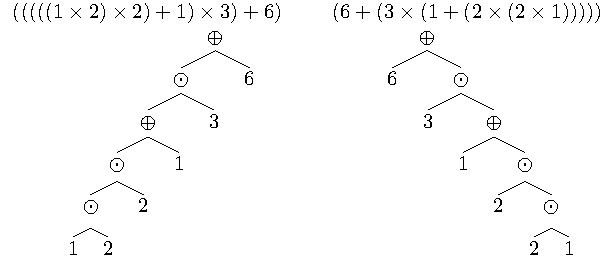
\includegraphics{../images/03-example-expression-syntax-tree-left-right.pdf}}
\caption{可线索化表达式的解析树}\label{fig:syntaxtree-left-right}
\end{figure}

可线索化表达式是指一类算术表达式,它的左支或者右支全部都是叶节点。这种表达式的求值过程是唯一的。向左或者向右展开完全是对称的,
向左展开的形式在求值时是从头计算到尾,向右展开的形式在求值时是从尾计算到头。这里我们取向左展开作为标准形式,记为 $\mathbb{T} \left [\mathbb{Q} \right ]$。

容易理解,有一种非常规范的线索化表达式,其中的乘法项和加法项交错出现,我们把这种可线索化表达式称为交错式。
任何一个可线索化表达式都可以通过适当添加加零项或者乘一项来补足成为交错式。因此交错式是可线索化表达式的一个典范形式。
我们记它为 $\mathbb{A} \left [\mathbb{Q} \right ]$。

\section{离散的自由生成群}\label{sec:freegroup}

我们考虑如下一个初始操作数,两个操作子生成的结构
\begin{itemize}
\item 初始操作数: $0$
\item 加法操作子: $\oplus_\mu: x \mapsto x + \mu$
\item 乘法操作子: $\otimes_\lambda: x \mapsto x \cdot e^\lambda$
\end{itemize}

在自由生成下,我们可以得到一个可线索化表达式上的群结构(注意是表达式上的,不是值上的群结构)。 在几何上看,这个生成过程得到一些由特定正交线族上的折线构成的路径。
下面我们考察这个自由群的交换子。有如下三种不同的引进方式。

\begin{equation}
x \oplus_\mu \otimes_\lambda \ominus_\mu \oslash_\lambda - x = \mu(1 - e^{-\lambda})\label{eq:commutator1}
\end{equation}

\begin{equation}
x \otimes_\lambda \oplus_\mu \oslash_\lambda \ominus_\mu - x = - \mu(1 - e^{-\lambda})\label{eq:commutator2}
\end{equation}

\begin{equation}
\tau = x \oplus_\mu \otimes_\lambda - x \otimes_\lambda \oplus_\mu = \mu(e^\lambda - 1)\label{eq:torsion}
\end{equation}

第三种方式比较对称,我们选择把它作为交换子的标准定义。因为直观上,正是这种加法和乘法上的不可交换性才造成了几何空间的扭曲,
我们把它称为“算术扭曲”并记为 $\tau$。 需要指出,因为对生成元的加乘操作被解释为几何上的路径,那么算术扭曲是一种定义在几何路径上的差量。

\begin{figure}[ht]
\centering
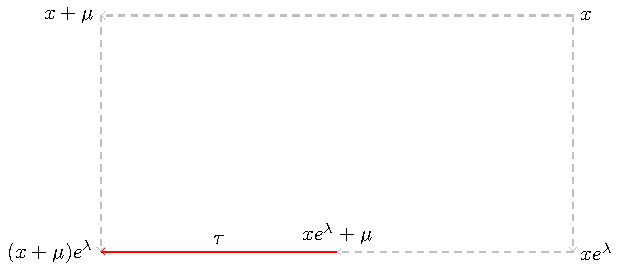
\includegraphics[width=0.7\textwidth]{../images/torsion}
\caption{算术扭曲作为几何路径上的差量}\label{fig:torsion}
\end{figure}

\section{流方程的形式解}

流方程刻画了一个双生成元的无穷小生成过程,它不是一个纯代数式的生成方式,而是一个几何式的过程。通过得到的微分方程,我们甚至可以纯形式地求出它的解析解。

从方程开始

$$
\frac{da}{ds} = \mu \cos \theta + a \lambda \sin \theta
$$

我们有

$$
\frac{1}{\lambda \sin \theta} \frac{d(\mu \cos \theta + a \lambda \sin \theta)}{\mu \cos \theta + a \lambda \sin \theta} = ds
$$

积分并化简得到

$$
\mu \cos \theta + a \lambda \sin \theta = e^{\lambda s \sin \theta} e^{C \lambda \sin \theta}
$$

考虑初始条件

$$
\mu \cos \theta + a_0 \lambda \sin \theta = e^{C \lambda \sin \theta}
$$

于是有

\begin{equation}
a = (a_0  + \frac{\mu}{\lambda} \cot \theta) e^{\lambda s \sin \theta} - \frac{\mu}{\lambda} \cot \theta
\end{equation}

对于给定的 $\theta$、$\mu$和$\lambda$,我们很容易可以验证这个形式解构成一个关于 $s$ 的单参数变换群,也即有:
\begin{itemize}
\item 变换合成:对任意的 $s_1$ 和 $s_2$,有 $a(a(a_0, s_1), s_2) = a(a_0, s_1 + s_2)$
\item 单位变换:$a(a_0, 0) = a_0$
\item 逆变换:$a(a(a_0, s), -s) = a_0$
\end{itemize}

\section{两种生成的兼容性}

从流方程的形式解出发,我们可以变形到一个特定形式,来考察赋值 $a$ 沿着 $\frac{\pi}{2}$ 的倍角方向的变化。

\[
a = (a_0  + \frac{\mu}{\lambda} \cot \theta) e^{\lambda s \sin \theta} - \frac{\mu}{\lambda} \cot \theta
\]

我们可以把这个式子变形为

\[
a =  a_0 e^{\lambda s \sin \theta} + \frac{\mu}{\lambda} (e^{\lambda s \sin \theta} - 1) \cot \theta
\]

应用 Taylor 展开和倍角公式,我们可以得到

\[
a = a_0 e^{\lambda s \sin \theta} + \mu s \cos \theta + \frac{\mu}{2\lambda} \sin 2\theta (\frac{\lambda^2s^2}{2!} + \frac{\lambda^3s^3}{3!} \sin \theta + \frac{\lambda^4s^4}{4!} \sin^2 \theta + \cdots)
\]

重新整理为下式

\begin{equation}
a = a_0 e^{\lambda s \sin \theta} + \mu s \cos \theta + \frac{\mu}{2\lambda} \Psi(s) \sin 2\theta
\end{equation}

很容易看出,当 $\theta$ 角取 $\frac{\pi}{2}$ 的倍数时, $\Psi(s)$ 不起作用,而是有:
\begin{itemize}
\item 当 $\theta = 0$ 时,$a = a_0 + \mu s$,编码了加法作用。
\item 当 $\theta = \frac{\pi}{2}$ 时,$a = a_0 e^{\lambda s}$,编码了乘法作用。
\item 当 $\theta = \pi$ 时,$a = a_0 - \mu s$,编码了减法作用。
\item 当 $\theta = \frac{3\pi}{2}$ 时,$a = a_0 e^{-\lambda s}$,编码了除法作用。
\end{itemize}

这告诉我们,只要 $a$ 满足流方程,那么 $a$ 就可以容纳\ref{sec:freegroup}节里的自由生成群的生成过程。而流方程本身就是刻画无穷小生成过程的微分方程,
所以,我们说无穷小生成兼容离散自由生成。

本节最后,让我们考察一下在 \ref{sec:arithmetic-expression} 小节定义的离散表达式的估值函数 $\nu$。
在离散的情况下,$\nu$ 是一个从表达式到值的映射,它是一个函数。而在流的观点下,可线索化表达式等价于路径,而 $\nu$ 就是一个函数,
它把路径映射为路径终点的赋值 $a$。

\section{算术表达式空间}



\newpage

\chapter{第一类空间}

\section{算术表达式空间}

张乐通过分离变量法得到了第一类算术表达式空间的解析解。我们对这个解析解进行了分析。在上半平面模型里,
不论加法生成元 $\mu$ 还是乘法生成元 $e^\lambda$ 的取值怎么变化,我们只需要变化空间的度规,赋值场 $a$ 始终是同一个解析解 $-\frac{x}{y}$。
此时,流方程是成立的。

![页二四](/curiosity/invitation/024.jpeg)

我们把如上情况下的几个数学对象综合到一起考虑作为一种更高层的数学对象:
* 实数域 $\mathbb{R}$
* 其上的可线索化表达式 $E[\mathbb{R}]$
* 所在的指定了度规的双曲空间$H$
* 标量的赋值场 $a$
* 所有的路径集合 $P$
* 路径集合可以解释为积分的集合 $I$

于是结构 $(\mathbb{R}, E[\mathbb{R}])$ 代表了这个数学对象的算术表达式的侧面;$(H, P)$ 代表了这个数学对象的几何侧面;
$(a, I)$ 代表了这个数学对象的分析学和函数论的侧面。

我们把这个综合的数学对象称为算术表达式空间。而如上设定的算术表达式空间是第一类的实例,称为第一类算术表达式空间。

\section{第一套网格}

![页二四](/curiosity/invitation/025.jpeg)

我们可以在双曲空间 $H$ 画出来由加法生成元和乘法生成元生成的离散的群的 Cayley 图。这个图能清晰的揭示局部结构怎么黏贴整合成一个整体的结构。
因为我们得到的离散的群是 Baumslag–Solitar 群,上图的模式在之前的研究中出现过。问题是,我们能把这个黏贴整合的过程写出来吗?怎么从四阶 Cayley 树粘合出上图?

\section{第二套网格}

另一个有趣的问题是,针对同一个算术表达式空间,上图是唯一的吗? 答案是否定的。

![页二四](/curiosity/invitation/026.jpeg)

我们还能找到另外一个 Cayley 图。这两个 Cayley 图不但作为图是同构的,而且还共享同一组梯度线-等值线坐标网。

![页二四](/curiosity/invitation/027.jpeg)

更有趣的是,它们能被一个共形变换联系起来。这不禁让我们思考:
* 为什么是这样两组 Cayley 图?它们有什么联系?背后有什么原因吗?
* 除了 Möbius 变换的写法,我们能用算术表达式的表征来写共形变换吗?比如,用某种算术表达式的变形,可以把这个共形变换写出来?

\section{变换的新写法}

平移、位似、反转

\section{算子的本征函数}

![页二四](/curiosity/invitation/028.jpeg)

为了展示这个领域在分析学和函数论方面的丰富性,我们指出赋值场 $a$ 是 Laplacian 的特征函数。但这是个普遍结论还是只在第一类算术表达式空间成立呢?
目前我们还不清楚。

\newpage

\chapter{进一步研究—几何篇}

\newpage

\chapter{进一步研究—分析篇}

\newpage

\chapter{进一步研究—计算篇}
\label{chap:computation}

\newpage

\chapter{进一步研究—复数化}

\newpage

\chapter{未解决的基本问题}

\newpage

\chapter{更加狂野的想象}

\newpage

\chapter{最后的总结}

\end{document}